\documentclass{article}
% Packages này giúp chúng ta gõ tiếng Việt trên LaTeX
\usepackage[utf8]{vietnam}
\usepackage{listings}
\usepackage{graphicx}
\graphicspath{ {./images/} }
\usepackage[acronym,nonumberlist]{glossaries}
\newacronym{WSNs}{WSNs}{Wireless Sensor Networks}
\newacronym{GPS}{GPS}{Global Positioning System}
\newacronym{EAs}{EAs}{Evolutionary Algorithms}
\newacronym{GAs}{GAs}{Genetic Algorithms}
\newacronym{SIOAs}{SIOAs}{Swarm Intelligence Optimization Algorithms}
\newacronym{NSGA-II}{NSGA-II}{Nondominated Sorting Genetic Algorithm II}
\newacronym{MOEA/D}{MOEA/D}{Multi-objective Evolutionary Algorithm based on Decomposition}
\newacronym{RL}{RL}{Reinforcement Learning}
\newacronym{DEs}{DEs}{Differential Evolution}

\title{Bài toán Tối ưu đa mục tiêu trong mạng cảm biến không dây}
\author{Trần Bảo Ngọc - HEDSPI IS K60}
\date{Tháng 11, 2019}

\begin{document}
\maketitle
\tableofcontents

\newpage
\section{Tổng quan}
\subsection{Mạng cảm biến không dây (\gls{WSNs}) là gì}
Mạng cảm biến không dây bao gồm số lượng lớn các nút cảm biến  không dây được triển khai trong một khu vực mục tiêu. Các nút này  có khả năng đo lường các thông số của môi trường, như:  nhiệt độ, độ ẩm, ánh sáng, âm thanh,.... Dữ liệu mà các cảm biến thu thập sẽ được truyền đi trên một kênh truyền thông không dây đến với trạm cơ sở. Trạm cơ sở  được cài đặt ứng dụng để xử lý và đưa ra các quyết định dựa trên các dữ liệu này.
\gls{WSNs} có một số đặc điểm chung với mạng tùy biến không dây (ad-hoc), do đó, nhiều khi nó chỉ được coi là một trường hợp đặc biệt của  mạng tùy biến không dây. Tuy nhiên, \gls{WSNs} có những đặc trưng rất riêng biệt như sau:
\begin{itemize}
    \item Các nút được triển khai với mật độ khá dày đặc, có thể cao hơn vài lần so với mạng tùy biến di động MANET. Điều này làm cho dữ liệu thu nhận được bới nhiều nút cảm biến khác nhau có sự tương đồng nhất định, gọi là sự dư thừa dữ liệu.
    \item Các nút thường được cumg cấp năng lượng bằng pin do chúng thường được triển khai tại những môi trương khắc nghiệt không thuận tiện cho việc sạc lại hay thay thế pin.
    \item Năng lượng, khả năng tính toán, dung lượng lưu trữ của các nút cảm biến là cực kỳ hạn chế.
    \item Mỗi mạng cảm biến không dây được thiết kế và triển khai đặc thù cho từng loại ứng dụng. 
    \item Các nút cả biến có tính tin cậy thấp, do điều kiện môi trường khắc nghiệt tại khu vực mục tiêu chúng có khả năng bị hỏng hóc, gặp lỗi khi đang hoạt động. Điều này cũng dẫn đến hình trạng (topo) của mạng thường xuyên thay đổi.
    \item Trong hầu hết các mạng, dữ liệu từ rất nhiều nút đều gửi về một trạm cơ sở duy nhất. Mô hình lưu lượng nhiều tới một (many-to-one) là đặc trưng của \gls{WSNs}.
\end{itemize}

Mạng cảm biến không dây được công nhận rộng rãi là một trong những công nghệ quan trọng nhất trong thế kỷ 21, có ứng dụng trên mọi lĩnh vực từ đời sống, sản xuất, quân sự. Rất nhiều nghiên cứu đang được tiến hành nhằm tiếp tục khai thác tiềm năng cũng như giải quyết các vấn đề, thách thức trong thiết kế và triển khai của công nghệ này. Trong tương lai gần, mạng cảm biến không dây sẽ có mặt ở khắp mọi nơi và thay đổi sâu sắc cuộc sống của chúng ta. 

\subsection{Cấu trúc của \gls{WSNs}}
Nội dung dưới đây được đươc viết dựa theo tài liệu \cite{architecture}
\subsubsection{Cấu trúc của một nút cảm biến}
Một node cảm biển thường bao gồm 4 thành phần: cảm biến, xử lý, truyền thông và bộ phận cung cấp năng lượng. 
\begin{figure}[ht]
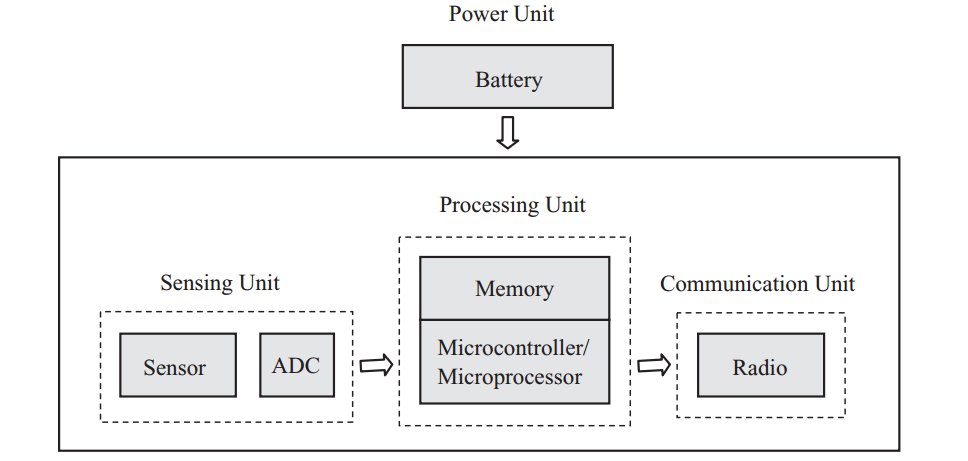
\includegraphics[width=\textwidth]{images/node-structure.PNG}
\caption{Cấu trúc một nút cảm biến \cite{architecture}}
\end{figure}
\newline Bộ phận cảm biến thường bao gồm một hoặc một vài cảm biến và các bộ chuyển đổi tương tự-số (ADC). Các cảm biển có nhiệm vụ giám sát các hiện tượng vật lý và sinh ra tín hiệu tương tự ứng với hiện tượng đó. Sau đó bộ chuyển đổi tương tự-số chuyển tín hiệu này thành tín hiệu số rồi đưa vào bộ xử lý trung tâm. 
\newline Bộ xử lý gồm một vi xử lý cùng với bộ nhớ, chịu trách nhiệm điều khiển mọi hoạt động của nút cảm biến, bao gồm cả xử lý những dữ liệu nhận được và đảm bảo kết nối với các nút khác trong mạng. Thay vì gửi toàn bộ dữ liệu gốc về trạm cơ sở để xử lý, một nút cảm biến sẽ tận dụng khả năng xử lý của chính nó để thực hiện các thao tác tính toán đơn giản và chỉ truyền dữ liệu cần thiết đã xử lý một phần. Bộ phận xử lý thường được thiết kế sao cho có thể hoạt động ở nhiều chế độ, ví dụ khi năng lượng còn lại ít, nó sẽ hạn chế tối đa các hoạt động của mình, nhằm tiết kiệm năng lượng .
\newline Bộ phận truyền thông có nhiệm vụ truyền và nhận dữ liệu thông qua kênh radio. Do năng lượng của một nút sensor là rất hạn chế nên bán kính truyền thông của nút cũng nhỏ. Một bộ phận truyển thông thường có 4 chế độ: truyền, nhận, rảnh (idle), ngủ. 
\newline Bộ phận nguồn sử dụng pin để cung cấp năng lượng, đảm bảo hoạt động của mọi thành phần khác, là một bộ phận rất quan trong trong mạng cảm biến không dây. Do mạng cảm biến không dây thường được triển khai ở những khu vực, địa hình khắc nghiệt nên việc sạc lại pin rất khó khăn. Vì vậy cần liên tục giám sát sự tiêu thụ năng lượng của các nút cảm biến. 
\newline Ngoài ra, tùy vào từng ứng dụng mà một nút cảm biến có thể được trang bị thêm một số thành phần khác. Ví dụ như đối với những ứng dụng yêu cầu cung cấp vị trí để hoạt động được thì cần trang bị thêm cho nút cảm biến hệ thống đinh vị toàn cầu \gls{GPS}. Một số mạng yêu cầu nút cảm biến có tính động thì cần trang bị thêm bộ di động cho các nút cảm biến, cung cấp khả năng di chuyển.
\newline Tất cả các thành phần này phải đủ nhỏ để chỉ chiếm 1 thể tích cỡ $1cm^3$ hoặc thậm chí nhỏ hơn. Đồng thời phải đáp ứng rất nhiều điều kiện khác như tiêu thụ năng lượng ở mức cực kỳ thấp, giá thành thấp, tự động, có khả năng thích nghi với môi trường,....
\subsubsection{Cấu trúc của \gls{WSNs}}
Một mạng cảm biến thường gồm một lượng lớn các nút cảm biển phân bố dày trong khu vực cần giám sát và một hoặc nhiều trạm cơ sở (gọi là data sink hay base station). Trạm cơ sở được đặt gần hoặc ngay bên trong vùng cảm biến. Trạm cơ sở gửi các yêu cầu truy vấn hoặc các lệnh đến các nút cảm biến, trong khi các nút cùng hoạt động để hoàn thành nhiệm vụ và gửi dữ liệu thu thập được đến trạm cơ sở. Vai trò của trạm cơ sở giống như là một gateway kết nối với các mạng ở bên ngoài (internet,...). Sau khi thu được dữ liệu từ các nút, nó thực hiện một số thao tác xử lý đơn giản rồi gửi thông tin liên quan hoặc dữ liệu đã qua xử lý thông qua Internet đến người dùng.
\newline Để gửi dữ liệu đi, các nút cảm biến có thể truyền trực tiếp đến trạm cơ sở mà không cần thông qua nút trung gian nào (truyền single-hop). Đặc điểm của cách truyền này, đồng thời là nhược điểm rất lớn của nó, đó là quãng đường truyền rất lớn, gây tốn kém về mặt năng lượng. Trong mạng cảm biến, năng lượng tiêu tốn cho truyền và nhận dữ liệu lớn hơn nhiều so với năng lượng dùng để cảm biến và tính toán. Ví dụ, để truyền 1 bit đến bộ thu cách 100m cần tiêu thụ lượng năng lượng tương đương với việc thực thi 3000 lệnh. Thêm vào đó, năng lượng truyền cần thiết tăng theo hàm mũ khi khoảng cách truyền tăng lên. Vì vậy cần có một phương thức để giảm lưu lượng  và khoảng cách truyền nhằm tiết kiệm năng lượng, kéo dài tuổi thọ của mạng
\newline Để đáp ứng mục tiêu này, phương thức kết nối multihop với khoảng cách ngắn rất được ưa chuộng. Trong hầu hết các mạng cảm biến, các nút được bố trí với mật độ cao, khoảng cách giữa các nút hàng xóm nhỏ. Mỗi nút gửi dữ liệu nó thu thập được về trạm cơ sở thông qua một hoặc một số nút trung gian, làm giảm năng lượng tiêu tốn cho việc gửi dữ liệu. Kiến trúc của một mạng multihop có thể chia làm 2 loại là kiến trúc phẳng (Flat architecture) và kiến trúc phân cấp (Hierarchical architecture)
\newline \emph{Kiến trúc phẳng}: các nút có vai trò ngang hàng, cùng thực thi nhiệm vụ cảm biến. Do số lượng nút là rất lớn, việc gán cho mỗi mỗi nút một đinh danh toàn cục (global identifier) rất khó khăn. Vì vậy, việc thu thâp dữ liệu thường được tiến hành bằng cách sử dụng định tuyến data-centric, tức là trạm cơ sở gửi truy vấn đến tất cả các nút bằng thuật toán tràn (flooding), chỉ có nút có dữ liệu mà trạm cơ sở yêu cầu sẽ phản hồi lại. Các nút kết nối đến trạm cơ sở sử dụng nút ngang hàng với nó như một nút trung gian chuyển tiếp dữ liệu.
\begin{figure}[ht]
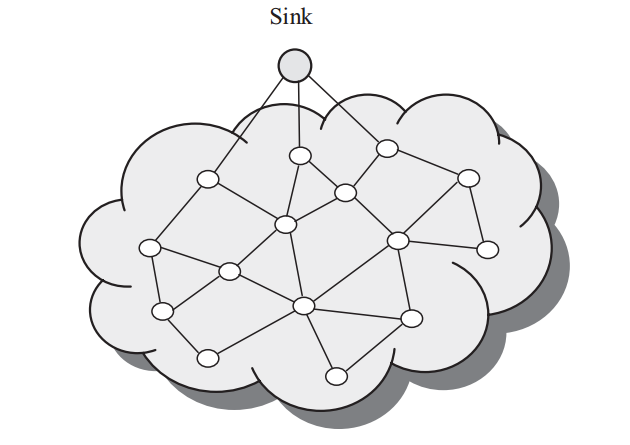
\includegraphics[width=\textwidth]{images/Flat.PNG}
\caption{Kiến trúc phẳng \cite{architecture}}
\end{figure}
\newline \emph{Kiến trúc phân cấp}: các nút cảm biến được phân thành các cluster, mỗi cluster có một cluster head. Tất cả các nút trong cluster gửi dữ liệu cảm biến được về cluster head của chúng, cluster head xử lý dữ liệu và gửi về trạm cơ sở. Một nút có năng lượng thấp chỉ phải thực hiện nhiệm vụ cảm biến và truyền ở khoảng cách ngắn về cluster head, ngược lại, nút có năng lượng cao được chọn làm cluster head phải thực thi việc xử lý dữ liệu và truyền xa. Quá trình này không chỉ giúp làm giảm năng lượng tiêu tốn cho việc truyền và nhận, mà còn giúp cân bằng tải, tăng khả năng mở rộng của mạng. Do các nút đều có khả năng truyền như nhau nên việc phân cụm cần được tiến hành định kỳ để cân bằng tải giữa các nút. Tại các cluster head có thể tiến hành tổng hợp dữ liệu (data aggregation) để giảm lượng dữ liệu cần truyền đến trạm cơ sở, tăng hiệu quả về mặt năng lượng của mạng.
\newline Vấn đề lớn nhất của kiến trúc phân cấp là cách phân chia cluster và cách chọn cluster head. Có nhiều chiến lược phân chia cluster khác nhau. Dựa vào khoảng cách từ cluster head tới các nút thành viên trong cluster, ta có kiến trúc phân cụm multi-hop và kiến trúc phân cụm single-hop. Dựa vào số tầng trong phân cấp các cụm (ví dụ, trong kiến trúc phân cụm 2 tầng, các cluster head tầng 1 gửi dữ liệu về các cluster head tầng 2, các cluster head tầng 2 chuyển tiếp dữ liệu về trạm sở), ta có kiến trúc phân cụm đơn tầng và đa tầng. 

\subsection{Các ứng dụng của \gls{WSNs}}
Các cảm biến có thể giám sát nhiều tham số vật lý, điều kiện, ví dụ như: ánh sáng, âm thanh, độ ẩm, áp suất, nhiệt độ, cấu tạo đất, chất lượng nước và không khí, các thuộc tính của một vật thể như kích cỡ, khối lượng, vị trí, tốc độ, phương hướng,....
Mạng cảm biến không dây có những ưu điểm vượt trội so với cảm biến có dây. Nó làm đơn giản hóa quá trình triển khai cũng như tối ưu chi phí, lại có thể được triển khai ở những địa hình khắc nghiệt, những nơi mà gần như là bất khả thi đối với cảm biến có dây. Ví dụ như trên chiến trường, ngoài không gian hay dưới biển. Mặc dù mạng cảm biến không dây ban đầu được thiết kế để phục vụ nhu cầu giám sát trong quân sự, nhưng với sự phát triển của công nghệ truyền không dây, giá thành cảm biến ngày càng rẻ thì mạng cảm biến không dây ngày càng phổ biến phục vụ cho cả 2 nhu cầu dân sự và quân sự. Ứng dụng cụ thể trong từng lĩnh vực được trình bày dưới đây theo tài liệu \cite{application}.
\subsubsection{Ứng dụng trong quân sự}
Mạng cảm biến không dây đóng vai trò quan trọng của các hệ thống chỉ huy, kiểm soát, liên lạc, điện toán, tình báo, giám sát, trinh sát và nhắm mục tiêu (C4ISRT) của quân đội.
\newline Chúng ta có thể nắm rõ được tình trạng của lực lượng, trang thiết bị bằng cách nhúng hoặc tích hợp vào các cảm biến. Các thông tin về trạng thái của phương tiện, vũ khí, lực lượng có thể được thu thập và chuyển tiếp đến cơ quan chỉ huy, nhằm đưa ra được quyết định tốt nhất. Dữ liệu của các đơn vị quân đội khác nhau cũng có được tập hợp và tổng hợp lại, tạo thành cái nhìn toàn cảnh về lực lượng quân đội toàn cầu.
\newline Trong các khu vực nhạy cảm, chúng ta có thể triển khai các mạng cảm biến không dây nhằm phát hiện sớm sự xâm nhập của địch bằng cách lập trình cho các cảm biển lập tức gửi đi thông báo về trạm cơ sở gần nhất khi phát hiện chuyển động.
\newline Trong chiến tranh hóa học và sinh học, chúng ta có thể triển khai các mạng cảm biến không dây như một biện pháp để phát hiện sớm sự xuất hiện của các chất độc hại trong môi trường và đưa ra cảnh báo kịp thời. Đồng thời, triển khai mạng cảm biến không dây trong khu vực bị tấn công bởi vũ khí hóa học và sinh học có thể cho phép chúng ta có những phân tích cụ thể, ví dụ như mức độ độc hại, chất độc còn tồn dư trong không khí, mà không cần đưa con người vào lấy mẫu.
\subsubsection{Ứng dụng trong môi trường}
Với mạng cảm biến không dây, việc thu thập những dữ liệu dài hạn trong tự nhiên ở một quy mô rộng lớn và chi tiết đã trở nên khả thi. Nhờ vậy, nó có rất nhiều ứng dụng trong lĩnh vực môi trường như phát hiện cháy rừng, giám sát môi trường sống, theo dõi động vật, hỗ trợ canh tác, giảm nhẹ tác hại thiên tai,....
\newline Ứng dụng mạng cảm biến trong giám sát môi trường sống cho phép các nhà nghiên cứu theo dõi môi trường sống của các loài động vật mà không gây ảnh hưởng đến chúng như các phương pháp truyền thống (cần sự can thiệp của con người). Có thể kể đến một dự án được triển khai trên đảo Greate Duck để quan sát các tổ của loài chim có tên gọi Leach’s Storm Petrels. Dự án của các nhà khoa học tại University of Hawaii dùng mạng cảm biến không dây để quan sát sự phát triển của các loài thực vật đang gặp nguy hiểm. Từ các dữ liệu thu thập được, họ xác định được đâu là yểu tố môi trường thúc đẩy sự phát triển của các loài thực vật này, từ đó đưa ra biện pháp bảo vệ chúng.
\newline Trong ứng dụng phát hiện cháy rừng, mạng cảm biến sẽ gửi cảnh báo cùng với vị trí chính xác của đám cháy đến nhà chức trách ngay khi đám cháy mới bắt đầu. Nhờ vậy, lực lượng cứu hỏa có thể nhanh chóng tiếp cận đám cháy trước khi nó không thể kiểm soát được. 
\newline Trong lĩnh vực canh tác, các cảm biến có thể được đặt trong lòng đất để thu thập các thông tin về tính chất của đất, hoặc cảnh báo khi các điều kiện của đất vượt quá một ngưỡng nào đó.
\subsubsection{Ứng dụng trong y tế - chăm sóc sức khỏe}
Mạng cảm biến không dây có nhiều ứng dụng trong y tế và chăm sóc sức khỏe, có thể kể đến ứng dụng theo dõi lượng đường trong cơ thể. Cảm biến có thể được cấy vào trong cơ thể người bệnh tiểu đường, thường xuyên thu thập dữ liệu về lượng đường và hiển thị lên một thiết bị đeo tay. Người bệnh luôn nắm bắt được sự tăng giảm của đường trong máu, nhận được cảnh báo nếu có sự thay đổi đột ngột để điều chỉnh thói quen sinh hoạt cho phù hợp. 
\newline Dự án SSIM (Smart Sensors and Integrated Microsystems) đang nghiên cứu phát triển võng mạc nhân tạo, với hi vọng sẽ giúp người mù có thể “nhìn” ở một mức độ chấp nhận được. Thiết bị sử dụng chip cảm biến thông minh bao gồm một mạch tích hợp (có khả năng truyền và nhận) và một loạt các cảm biến. Những thách thức trong ứng dụng này bao gồm thiết lập một liên kết giao tiếp giữa võng mạc được cấy ghép và máy tính bên ngoài để xác định xem hình ảnh có được nhìn thấy chính xác hay không. Điều chỉnh lượng điện năng được sử dụng bởi hệ thống để tránh tổn thương võng mạc và các mô xung quanh cũng là một mối quan tâm lớn.
\subsubsection{Ứng dụng trong công nghiệp sản xuất}
Trong công nghiệp, mạng cảm biến không dây được sử dụng để giám sát quá trình sản xuất hoặc tình trạng của các thiết bị sản xuất. Ví dụ, các nhà máy hóa chất hoặc nhà máy lọc dầu sử dụng cảm biến để giám sát tình trạng của các đường ống dẫn dài hàng kilomet. Các cảm biến siêu nhỏ được tích hợp vào các bộ phận máy móc mà con người không thể kiểm tra được  để thường xuyên giám sát trạng thái của các bộ phận này và gửi cảnh báo ngay khi có trục trặc. Theo các phương pháp truyền thống thì các cuộc kiểm tra thiết bị được tiến hành định kỳ, rất tốn kém (theo thống kê, các nhà sản xuất thiết bị công nghiêp tiêu tốn hàng tỷ đô cho việc bảo trì mỗi năm). Với mạng cảm biến không dây, chúng ta chỉ cần tiến hành kiểm tra dựa vào tình trạng của thiết bị, giúp giảm chi phí bảo trì, tăng tuổi thọ của máy móc, thậm chí giảm tai nạn lao động do hỏng hóc của máy móc.
\subsubsection{Ứng dụng trong nhà thông minh}
Mạng cảm biến không dây có khả năng làm cho cuộc sống của  con người tiện nghi hơn.
\newline Nhà thông minh: Mạng cảm biến được tích hợp vào nhà ở, hình thành một mạng tự trị. Ví dụ, một chiếc tủ lạnh thông minh được kết nối với lò vi sóng hoặc bếp thông minh sẽ chuẩn bị thực đơn dựa trên những nguyên liệu có sẵn trong tủ lạnh đó, sau đó gửi các tham số phục vụ việc nấu nướng đên bếp hoặc lò vi sóng. Lịch chiếu phim, nội dung các đĩa CD. DVD cũng có thể được kiểm soát và điều khiển từ xa để phù hợp nhu cầu các thành viên trong gia đình
\newline Đo lường từ xa: Sử dụng mạng cảm biến không dây, các số đo về nước, ga, điện trong nhà có thể dễ dàng thu thập và gửi đến một trung tâm dữ liệu thông qua mạng không dây
\subsection{Các vấn đề trong mạng cảm biến không dây}
Có rất nhiều thách thức và vấn đề cần xem xét trong thiết kế và triển khai mạng cảm biến không dây. Trong phạm vi đồ án, em xin được trình bày về các vấn đề sau: tuổi thọ của mạng, bao phủ và kết nối trong mạng. Vấn đề tuổi thọ của mạng được viết dựa theo tham khảo từ tài liệu \cite{dietrich2009lifetime}, vấn đề bao phủ và kết nối được viết dựa theo tài liệu \cite{fan2010coverage}
\subsubsection{Tuổi thọ của mạng cảm biến không dây}
Tuối thọ của mạng có thể nói là số đo quan trọng nhất khi đánh giá một mạng cảm biến, phụ thuộc mật thiết vào tuổi thọ của mỗi nút tạo nên mạng. Tuổi thọ của mạng cần được nghiên cứu và đánh giá kỹ lưỡng do đặc điểm của mạng cảm biến không dây thường được triển khai tại những khu vực nguy hiểm và khắc nghiệt cùng với số lượng nút cảm biến rất lớn, do đó việc sạc lại hoặc thay thế các nút cảm biến là rất khó khăn, thậm chí là bất khả thi. 
\newline Có rất nhiều nghiên cứu liên quan đến thời gian sống của mạng cảm biến không dây, dẫn đến rất nhiều các định nghĩa khác nhau cùng tồn tại. Dưới đây là một số định nghĩa hay được sử dụng:
\begin{itemize}
    \item \emph{Dựa trên số lượng nút sống: }
    Tuổi thọ của mạng được định nghĩa là khoảng thời gian từ lúc bắt đầu đến khi có một nút chết, tức là: $T^{n}_{n} = minT_{v}$ với $T_{v}$ là thời gian sống của nút $v$. Một số tác giả không bao gồm thời gian sống của trạm cơ sở trong công thức trên, với giả sử là tại đó luôn được cung cấp năng lượng. Với định nghĩa này, việc tính toán thời gian sống của mạng rất đơn giản và không phải cân nhắc tới các vấn đề xảy ra do topo của mạng thay đổi khi có  nút chết. Tuy nhiên, định nghĩa này là không phù hợp với các mạng có tính dư thừa, tức là các mạng vẫn có thể hoạt động được khi có một nút chết. Đồng thời, nó cũng chưa xem xét vấn đề hỏng hóc phần cứng của mạng cảm biến không dây có thể xảy ra từ rất sớm do điều kiện môi trường, làm tuổi thọ của mạng nếu được đo đạc theo cách này sẽ bị rút ngắn một cách nghiêm trọng.  Định nghĩa này chỉ phù hợp với các mạng mà trong đó các nút có vai trò quan trọng ngang nhau, đều không thể thiếu đối với sự hoạt động ổn định của mạng.
    Định nghĩa thời gian sống dựa trên số lượng nút sống thường được sử dụng trong các thuật toán có mục tiêu tối đa hóa thời gian sống của mỗi nút, hoặc các nút sẽ cạn kiệt năng lượng gần như là cùng lúc với nhau.
    \newline Một số biến thể khác của $T^{n}_{n}$ là $T^{k}_{n}$ định nghĩa thời gian sống của mạng từ lúc bắt đầu đến tỷ lệ nút còn sống nhỏ hơn một ngưỡng $\beta$ nào đó, tức là khoảng thời gian trong đó có ít nhất $k$ nút còn sống. Ngoài ra, có thể chia các nút cảm biến thành hai tập, tập gồm các  nút thiết yếu và tập các  nút không thiết yếu. Tập các nút không thiết yếu có thể chịu được $k$ nút chết, còn tập các nút thiết yếu  không thể chịu được nút chết nào. 
    \item \emph{Dựa trên bao phủ của mạng: }
    Tuổi thọ của mạng là khoảng thời gian mà khu vực cần giám sát được bao phủ hoàn toàn (nằm hoàn toàn trong phạm vi cảm biến của ít nhất một nút cảm biến). Một số biến thể khác chỉ cần một phần của khu vực được bao phủ, hoặc toàn bộ khu vực cần nằm trong phạm vi cảm biến của ít nhất $k$ nút cảm biển.
    Vấn đề bao phủ cũng là một vấn đề quan trọng trong mạng cảm biến không dây, tuy nhiên định nghĩa tuổi thọ chỉ dựa vào khái niệm bao phủ có thể sẽ chưa đầy đủ trong nhiều bài toán bởi nó không đảm bảo được đữ liệu có thể được truyền về trạm cơ sở.
    \item \emph{Dựa trên kết nối: }
    Một số tác giả đã định nghĩa tuổi thọ của mạng  bằng tổng số gói tin được truyền đến trạm cơ sở. Cách định nghĩa này có hạn chế là nó rất phụ thuộc vào thuật toán được sử dụng trong mạng. Nếu mạng sử dụng các thuật toán tổng hợp dữ liệu, số gói tin được gửi sẽ giảm đi so với các mạng không sử dụng các giải thuật tổng hợp dữ liệu, mặc dù lượng thông tin được gửi là tương đương nhau.
    Một số tác giả khác định nghĩa thời gian sống của mạng thông qua số vòng gửi nhận dữ liệu thành công, với điều kiện ràng buộc không có nút chết trong các vòng gửi nhận dữ liệu. Điều này làm cho cách định nghĩa này có thêm các nhược điểm của cách định nghĩa $T_n^n$ đã trình bày ở trên.
    Kết hợp vấn đề kết nối khi định nghĩa thời gian sống là điều cần thiết, tuy nhiên,  cần xem xét cả kết nối đến trạm cơ sở, thay vì chỉ xét đến kết nối giữa hai  nút cảm biến bất kỳ.
\end{itemize}
Khi đánh giá tuổi thọ của mạng, cần xem xét các vấn để sau:
\begin{itemize}
    \item \emph{Khả năng di chuyển của các nút và sự thay đổi hình trạng mạng}
\newline Tính động của các nút đem đến nhiều khả năng mới cho mạng cảm biến không dây, như cải thiện độ bao phủ và tính kết nối của mạng, tuy nhiên cũng đem đến nhiều thách thức, khó khăn trong việc kiểm soát mang cũng như đánh giá thời gian sống của mạng cảm biến. 
\newline Khi nút cảm biến di chuyển, một vài kết nối có thể bị mất đi hoặc được tạo ra thêm, vùng bao phủ cũng thay đổi, tương tự với trường hợp khi có nút chết trong mạng. Các yếu tố môi trường, địa hình cũng ảnh hưởng đến topo mạng. Ví dụ, nút cảm biến có thể bị rơi xuống vực, bị di chuyển một cách vô tình hoặc cố ý, có thể do các loại động vật trong khu vực mang đi. Do đó, ngay cả trong các mạng cảm biến không dây có tính chất tĩnh (các nút không có khả năng di chuyển) cũng cần xem xét cả vấn đề này. Nếu không xem xét thật cẩn thận vấn đề này, mạng có thể có tuổi thọ cực kỳ ngắn, gây lãng phí thời gian và tiền bạc.
\item \emph{Tính đa dạng}
\newline Hầu hết các mô hình đều giả sử rằng các nút cảm biến là hoàn toàn giống nhau, trong khi một số khác mới chỉ xem xét sự đa dạng trên một hoặc hai phương diện. Tuy nhiên, một nghiên cứu đã chỉ ra rằng có ít nhất 8 đến 10 loại khi nói đến sự đa dạng của các nút cảm biến trong một mạng, có ảnh hưởng lớn đến hoạt động và tuổi thọ mạng.
\newline Phổ biến nhất là việc phân chia năng lượng của các nút thành 2 loại, các nút có mức năng lượng nhỏ và một số ít các nút có mức năng lượng cực kỳ lớn, có thể là vô tận. Sự đa dạng về mức năng lượng này thường được áp dụng trong kiến trúc phân cụm, với các cluster head là các nút có năng lượng rất lớn.
\newline Một số mô hình xem xét sự đa dạng trong bán kính truyền thông. Bán kính truyền thông có thể bị thay đổi và có các hình dạng bất thường thay vi luôn luôn là hình cầu do sự ảnh hưởng của thời tiết. Hoặc trong kiến trúc phân cụm, cluster head có thể có bán kính truyền thông lớn hơn do cần truyền khoảng cách dài đến trạm cơ sở. 
\newline Tính đa dạng của các nút có ảnh hưởng rất lớn đển thời gian sống của mạng, nó có thể kéo dài thời gian sống đối với mạng có các nút có mức năng lượng lớn, hoặc làm giảm đi nếu có những nút phải thực hiện quá nhiều nhiệm vụ.
    \item \emph{Cách triển khai}
    \newline Đích đến của các gói tin ảnh hưởng đến việc truyền và nhận trong mạng. Ngoài những trường hợp đơn giản chỉ có một trạm cơ sở được đặt cố định ở giữa hoặc biên của mạng, còn có những trường hợp phức tạp hơn với nhiều trạm cơ sở được đặt ở nhiều vị trí khác nhau, thậm chí các trạm này còn có thể di chuyển được. Điều này dẫn đến các phương thức truyền thông khác nhau, mức tiêu thụ năng lượng cũng khác nhau
\end{itemize}

\subsubsection{Vấn đề bao phủ  trong mạng cảm biến không dây}
Bao phủ là một đề tài nghiên cứu nền móng trong mạng cảm biến không dây, là một trong những yếu tố để đánh giá chất lượng mạng cảm biến. Vấn đề bao phủ thường được nghiên cứu kết hợp cùng nhiều vấn đề khác, trong đó quan trọng nhất là thiết kế một mô hình  bao phủ hiệu quả trong khi duy trì được tính kết nối và tối ưu hóa thời gian sống của mạng.
\newline Có rất nhiều yếu tố ảnh hưởng đến độ bao phủ của mạng cảm biến không dây, tuy nhiên một số yếu tố có ảnh hưởng lớn có thể kể đến là:
\begin{itemize}
    \item Chiến lược triển khai: có hai loại là ngẫu nhiên và xác định trước. Với cách triển khai xác định trước, số lượng nút cảm biến, vị trí đặt cảm biến,... có thể được tính toán trước. Mô hình này áp dụng cho mạng cỡ từ nhỏ tới trung bình trong môi trường bình thường. Ngược lại, phương án triển khai ngẫu nhiên phù hợp với các môi trường có lực lượng thù địch, có địa hình khó tiếp cận, có thiên tai thảm họa,... và có số lượng nút lớn. Với các điều kiện này, việc tính toán trước số lượng nút và vị trí nút là bất khả thi. Do đó, các nút cảm biến được rải ngẫu nhiên trên khu vực cần quan sát bằng cách dùng máy bay để rải rác.
    \item Mô hình cảm biến: có hai loại chính là nhị phân và xác suất. Trong mô hình nhị phân, các nút có bán kính cảm biến cố định $r$, và chúng có thể cảm biến được các sự kiện xảy ra trong phạm vi cảm biến đó với xác suất 100\%.
    \begin{equation}
        c_{xy}(s_i) = 
        \begin{cases}
            1 & \text{ Nếu } d(s_i, p) < r \\
            0 & \text{ Ngược lại}
        \end{cases}
    \end{equation}
    Tuy nhiên trong thực tế, cảm biến không phải luôn chính xác. Trong mô hình xác suất, xác suất phát hiện được sự kiện hay vật thể và độ nhạy của nút cảm biến sẽ giảm khi khoảng cách tăng.
    \begin{equation}
        c_{xy}(s_i) = 
        \begin{cases}
            0 & \text{ Nếu } d(s_i, p) \geq r+r_e \\
            e^{-\lambda\alpha^\beta} & \text{ Nếu } r-r_e < d(s_i, p) < r+r_e \\
            1 & \text{ Nếu } d(s_i, p) \leq r-r_e
        \end{cases}
    \end{equation}
    $r_e < r$ biểu diễn mức độ không chắc chắn trong việc phát hiện sự kiện của nút cảm biến. $\alpha = d(s_i, p) - (r-r_e)$, $\beta$ và $\lambda$ là các tham số đo xác suất phát hiện khi điểm mục tiêu cách nút cảm biến một khoảng lớn hơn $r_e$.
    \item Phạm vi truyền thông: các nút cảm biến thông thường có bán kính truyền thông không thay đỏi nhưng cũng có các cảm biến có khả năng thay đổi mức năng lượng để thay đổi bán kính truyền thông trong các thời điểm khác nhau. Thực tế, phạm vi truyền thông còn bị ảnh hưởng bởi nhiều yếu tố như độ cao của cảm biến, các vật cản.
    \item Đặc trưng của thuật toán: Khi mạng được triển khai, một thuật toán bao phủ được tiến hành để xác định xem khu vực mục tiêu đã đạt được mức độ bao phủ cần thiết hay chưa. Trong mô hình tập trung, thuật toán bao phủ được thực thi ở một nút trung tâm, do đó, thông tin từ tât cả các nút phải được gửi tới nút trung tâm này. Trong mô hình phân tán, thuật toán bao phủ được thực thi tại tất cả các nút dựa vào thông tin có được từ một số nút hàng xóm. Mô hình tập trung có khả năng cung cấp thông tin một cách chính xác và đầy đủ hơn cho thuật toán bao phủ nhưng lại tiêu tốn lượng lớn năng lượng cho việc truyền dữ liệu.
    \item Khả năng di chuyển của nút cảm biến: Các nút cảm biến có khả năng di chuyển đem lại nhiều lợi ích lớn, ví dụ như khả năng cải thiện hoặc duy trì độ bao phủ của mạng.
\end{itemize}
Vấn đề bao phủ được chia làm ba loại:
\begin{itemize}
\item \emph{Bao phủ khu vực}: Mục tiêu chính của mạng là bao phủ được một khu vực (tập tất cả các điểm nằm trong trường cảm biến) và mọi điểm thuộc khu vực đó đều cần được giám sát.
\item  \emph{Bao phủ điểm mục tiêu}: Mục tiêu là bao phủ một tập các điểm mục tiêu có vị trí đã biết trước. Bao phủ điểm tập trung vào việc xác định vị trí chính xác để triển khai các nút cảm biến, đồng thời bảo đảm bao phủ hiệu quả đối với một tập có số lượng giới hạn các điểm mục tiêu tĩnh. Một cách tổng quát, đây có thể coi là trường hợp đặc biệt của bao phủ khu vực.
\begin{figure}[ht]
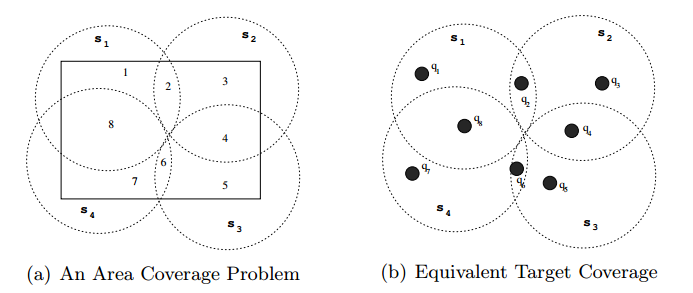
\includegraphics[width=\textwidth]{images/coverage.png}
\caption{Mối quan hệ giữa bao phủ khu vực và bao phủ mục tiêu \cite{thai2008coverage}}
\end{figure}
\item  \emph{Bao phủ đường}: Mục tiêu chính là tối đa hóa hoặc tối thiểu hóa khả năng xâm nhập vào một khu vực nào đó.
\end{itemize}
Một số vấn đề khác thường được nghiên cứu là bài toán k-coverage, yêu cầu mỗi điểm $q$ nằm trong khu vực mục tiêu $A$ phải được giám sát bởi ít nhất $k$ cảm biến ($k > 1$). Vấn đề này được nghiên cứu nhằm phục vụ cho các trường hợp, ứng dụng yêu cầu sự giám sát rất chặt chẽ, ví dụ như giám sát trong quân sự. Hoặc một số ứng dụng cần đồng thời nhiều nút cảm biến mới có thể phát hiện được sự kiện nào đó, ví dụ như giao thức định vị dựa trên ba đỉnh của hình tam giác cần $k \geq 3$ để giám sát mục tiêu di động.  Để kiểm tra được toàn bộ khu vực $A$ đã đạt được k-coverage hay chưa, cách đơn giản nhất là chia $A$ thành các khu vực con và kiểm tra từng khu vực con này đã đạt k-coverage hay chưa. Có thể phân chia theo phạm vi cảm biển của các nút (ví dụ chia thành $n$ hình tròn bán kính $r$). Tuy nhiên, việc phân chia và quản lý một số lượng lớn các khu vực con là rất khó khăn, tốn kém. Các tác giả trong \cite{huang2005coverage} đã chứng minh được rằng: Khu vực $A$ đạt được$k$-coverage khi và chỉ khi tất cả các điểm thuộc đường chu vi cảm biến của mọi nút  đều được bao phủ bởi ít nhất $k$ cảm biến.

\subsubsection{Vấn đề kết nối trong \gls{WSNs}}
Một vấn đề quan trọng khác của \gls{WSNs} là kết nối. Một mạng cảm biến không dây có thể mô hình hóa thành một đồ thị, với các đỉnh là các nút cảm biến và các cạnh là các kết nối giữa các cặp nút cảm biển. Một nút cảm biến $s_i$ có thể kết nối trực tiếp đến nút $s_j$ nếu $d(s_i, s_j)\leq R_c $, tức là $s_i$ nằm trong phạm vị truyền thông của nút $s_j$. Nếu tất cả các nút của mạng đều có thể liên lạc trực tiếp hay gián tiếp về trạm cơ sở, ta nói mạng đảm bảo được kết nối. Đồ thị sinh ra từ mạng cảm biến như vậy là đồ thị liên thông. 
\newline Luôn đảm bảo tính kết nối là yêu cầu quan trọng trong \gls{WSNs}, giúp cho dữ liệu được lan truyền về trạm cơ sở một cách kịp thời, chính xác. Có thể nói thời gian sống của mạng kết thúc khi nó bị mất tính kết nối. Để chắc chắn một nút cảm biến luôn được đặt trong bán kính cảm biến của ít nhất một nút khác, và tránh đặt hai nút quá gần nhau, ta có thể thực hiện tối thiểu hóa phép toán sau:
\begin{equation*}
    f_{con} = \sum_{i=1}^n 1-e^{-(R_{c_i}-R_{s_i})}
\end{equation*}
Mối quan hệ bao phủ - kết nối trong mạng cảm biến không dây: Các tác giả trong \cite{zhang2005maintaining} đã đưa ra một định lý quan trọng về mối quan hệ giữa bao phủ và kết nối là: 
\newline \emph{Định lý}: Nếu các cảm biến được triển khai trong một khu vực là hữu hạn, điều kiện cần và đủ để phủ sóng toàn bộ khu vực mà vẫn đảm bảo tính kết nối là  $ R\geq 2r$ với $R$ là bán kính truyền thông, $r$ là bán kính cảm biến. Nói cách khác, khi $ R\geq 2r$, mạng sẽ được đảm bảo về tính kết nối, ta chỉ cần tập trung điều chỉnh sao cho bảo đảm về mặt bao phủ.
\newline Để tăng tính chịu lỗi cho \gls{WSNs}, mô hình k-connectivity cũng thường được xem xét. Trong đó, một nút cảm biến phải nằm trong bán kính cảm biển của ít nhất $k$ nút khác. Đồ thigj sinh ra từ mạng như vậy là một đồ thị k-liên thông ($k$-connected graph). Nhờ vậy, khi trong mạng có ít hơn hoặc bằng $k-1$ nút chết, mạng vẫn có thể hoạt động bình thường. Mạng chịu lỗi tốt hơn, thời gian sống cũng được kéo dài hơn. 
\newline Các tác giả trong \cite{tian2005connectivity} đã chứng minh định lý quan trọng sau về mối quan hệ giữa mức độ bao phủ với mức độ kết nối:
\newline \textbf{Định lý: } Một tập các nút cảm biển $k$-bao phủ khu vực mục tiêu tạo thành đồ thị $k$-liên thông nếu $R_c \geq 2R_s$.

\subsection{Bài toán tối ưu}
\subsubsection{Khái niệm và phân loại bài toán tối ưu}
Bài toán tối ưu là bài toán đi tìm các giá trị tham số liên quan sao cho hàm mục tiêu đạt giá trị nhỏ nhất hoặc lớn nhất. Bài toán tối ưu có vai trò quan trọng trong mọi mặt của cuộc sống. Bởi vì, trong thực tế, các tài nguyên đều hữu hạn nên cần tìm cách sử dụng chúng sao cho hiệu quả nhất.
\newline Bài toán tối ưu có thể viết dưới mô hình toán học như sau:
\newline Cho $f: X \rightarrow R $ với X là không gian nào đó. 
\newline Mục tiêu: Maximize/minimize $f(x)$ với ràng buộc $ X \in D  \subset X  $, trong đó:
\begin{itemize}
    \item $f(x)$ là hàm mục tiêu
    \item $X$ là không gian chấp nhận được
    \item $D$ là miền chấp nhận được hoặc miền ràng buộc
    \item $x \in D$ là nghiệm chấp nhận được
    \item Điểm $ x^\ast$ gọi là nghiệm toàn cục nếu  tại đó f(x) nhận giá trị tối ưu, tức là $ f(x^\ast) \geq f(x),  \quad \forall X \in D$ hoặc  $ f(x^\ast) \leq f(x),  \quad \forall X \in D$
    \item Nếu $D = X$ thì bài toán tối ưu không ràng buộc, ngược lại là bài toán tối ưu có ràng buộc
    \item Điều kiện $ x \in D $ thường xuất hiện dưới các dạng:
    \begin{itemize}
        \item Đẳng thức
        \item Bất đẳng thức
        \item Bao hàm thức
    \end{itemize}
\end{itemize}
Dựa vào các tiêu chí khác nhau, ta có các cách phân loại bài toán tối ưu như sau:
\begin{itemize}
    \item Tối ưu rời rạc (tối ưu tổ hợp)  và tối ưu liên tục: Miền chấp nhận được là một tập các giá trị rời rạc. Đặc biệt, nếu là tập các giá trị nguyên, ta có bài toán Quy hoạch nguyên.
    \item Tối ưu có ràng buộc và tối ưu không có ràng buộc: Nếu D = X thì bài toán tối ưu không ràng buộc, ngược lại là bài toán tối ưu có ràng buộc. Tối ưu có ràng buộc có thể được phân chia thành nhiều nhánh nhỏ khác phụ thuộc vào đặc điểm của ràng buộc, bao gồm tối ưu tuyến tính (hàm mục tiêu và  các hàm ràng buộc đều là hàm tuyến tính) và tối ưu phi tuyến  (hàm mục tiêu và  các hàm ràng buộc đều là hàm phi tuyến). Trong tối ưu phi tuyến còn bao gồm tối ưu trơn. tối ưu lồi và tối ưu không lồi. Hệ ràng buộc cũng rất đa dạng như đã trình bày ở trên.
    \item Tối ưu đơn mục tiêu và tối ưu đa mục tiêu: Tùy thuộc vào số lượng hàm mục tiêu là một hay nhiều hàm không hòa hợp nhau, ta có thể  phân chia bài toán tối ưu thành đơn hay đa mục tiêu. Tối ưu đa mục tiêu là bài toán quan trọng trong \gls{WSNs}, định nghĩa, phương pháp giải sẽ được trình bày chi tiết hơn ở mục 1.5.2.
    \item Tối ưu ngẫu nhiên và tối ưu xác định: Trong bài toán tối ưu xác định, tất cả các biến của bài toán đều là biến xác định. Trong bài toán tối ưu ngẫu nhiên, một vài hoặc tất cả các biến, tham số của bài toán không có giá trị xác định mà được mô tả dưới dạng xác suất. 
\end{itemize}
\subsubsection{Các phương pháp giải bài toán tối ưu đa mục tiêu}
Trong mạng cảm biến không dây, bài toán tối ưu hóa đa mục tiêu rất được chú trọng, do mạng cảm biến không dây là mạng có rất nhiều ràng buộc và yếu tố phụ thuộc lần nhau cần xem xét khi thiết kế và triển khai. Do đó, em xin trình bày một số phương pháp giải bài toán tối ưu đa mục tiêu.
\newline Một bài toán tối ưu đa mục tiêu với $n$  biến và $m$ mục tiêu có mô hình toán học như sau:
 $$min f(x) = min[f_1(x), f_2(x),..., f_m(x)]$$
 $$\text{s.t. } g_i(x) \leq 0,  \quad i = 1, 2,.., m \text{,}$$
 $$h_j(x) = 0,   \quad j = 1, 2,..., m $$
\newline $x \in R^n$ là không gian quyết định, $f(x) \in R^m$ là không gian mục tiêu. Trong thực tế, các hàm mục tiêu có thể bị đụng độ với nhau, tức là khi giá trị $f_i(x)$ tăng lên thì $f_j(x)$ bị giảm đi. Do đó, nghiệm tối ưu toàn cục có thể không tồn tại. Thay vào đó, ta sẽ cố gắng đạt được tối ưu Pareto. Một số khái niệm liên quan đến tối ưu Pareto:
\begin{itemize}
    \item Thống trị Pareto: Một lời giải $a$ được gọi là thống trị lời giải $b$ nếu:
    \begin{itemize}
        \item $f_i(a) \leq f_i(b) \quad \forall i \in \{1, 2,..., m\}$
        \item $f_i(a) < f_i(b) \quad  \exists  i \in \{1, 2,..., m\}$
    \end{itemize}
    \item Tối ưu Pareto: Lời giải $a$ được gọi là điểm tối ưu Pareto nếu không tồn tại lời giải $b \in R^n$ thống trị lời giải  $a$. Tập tất cả các điểm tối ưu Pareto trong miền quyết định gọi là  Pareto-optimal set (PS). Ảnh của tập PS trong miền mục tiêu gọi là biên Pareto (Pareto-front - PF)
\end{itemize}
\begin{figure}[ht]
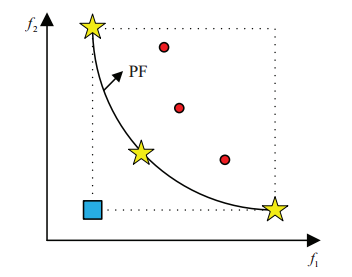
\includegraphics[width=\textwidth]{images/pareto.PNG}
\caption{Biên pareto với bài toán tối ưu hai mục tiêu không có ràng buộc \cite{fei2016survey}}
\end{figure}
Các thuật toán giải bài toán đa mục tiêu \cite{fei2016survey}
\newline Các phương pháp mở rộng dựa trên quy hoạch toán học
\begin{itemize}
    \item Phương pháp tổng trọng số tuyến tính: Phương pháp này biến một bài toán đa mục tiêu về đơn mục tiêu bắng cách gán trọng số cho mỗi biến số để có được một hàm đánh giá. Biên Pareto thu được bằng cách giải nhiều bài toán đơn mục tiêu này, mỗi bài toán tương ứng với một vectơ trọng số khác nhau. Lưu ý cần chuẩn hóa các biến số trước khi đưa vào hàm đánh giá.
    \item Phương pháp ràng buộc $\epsilon$: Phương pháp này đưa bài toán đa mục tiêu về đơn mục tiêu bằng cách chọn ra 1 hàm mục tiêu duy nhất để tối ưu hóa, $n-1$  hàm mục tiêu còn lại đóng vai trò như các ràng buộc. Phương pháp này thường không hiệu quả đối với các bài toán có nhiều hơn hai mục tiêu.
    $$ min f_i(x) $$
    $$ f_j < \epsilon_j \text{,} \quad j \neq i$$
    $$ H(x) = 0, \quad G(x) \leq 0$$
\end{itemize}
Các giải thuật metaheuristic lấy ý tưởng từ tự nhiên: Hầu hết các phương pháp tối ưu hóa cổ điển bị ràng buộc với một số lượng giới hạn các cấu trúc toán học chuẩn nào đó. Nhưng trong thực tế, việc đưa được các hiện tượng, vấn đề về mô hình tối ưu chuẩn rất khó khăn. Thêm vào đó, có nhiều yếu tố khiến việc tính toán trở nên khó khăn như số lượng biến số quá lớn, tính phi tuyến,... Vì vậy các phương pháp quy hoạch toán học cổ điển có thể không phù hợp với các vấn đề thực tiễn xảy ra trong \gls{WSNs}.
\newline So với các phương pháp toán học cổ điển, phương pháp metaheuristic ít bị ảnh hưởng bởi mô hình toán học của bài toán, tuy nhiên, chi phí tính toán tăng lên khi cần độ chính xác cao hơn. Các giải thuật tối ưu dựa trên metaheuristic được chia làm 2 nhánh là nhóm các giải thuật tiến hóa (\gls{EAs}) và nhóm các giải thuật dựa trên trí tuệ bầy đàn (\gls{SIOAs})
\newline \emph{Các giải thuật tiến hóa}: \gls{EAs} thuộc họ các giải thuật tìm kiếm ngẫu nhiên, dựa trên ý tưởng từ sự chọn lọc và tiến hóa trong tự nhiên. Mục tiêu của EAs là tìm kiếm các lời giải  gần như là tối ưu trong toàn cục bằng cách lặp lại việc đánh giá các hàm mục tiêu qua nhiều thế hệ.
\begin{itemize}
    \item Giải thuật di truyền (\gls{GAs}): Dựa trên lý thuyết về tiến hóa và di truyền, với những ưu điểm vượt trội so với các phương pháp truyền thống. GAs có thể sử dụng để giải quyết hầu như mọi loại bài toán tối ưu, thuận tiện cho tính toán song song.
    \newline GAs bao gồm 6 bước chính:
    \begin{itemize}
        \item Khới tạo: Khởi tạo quần thể với $n$ cá thể
        \item Đánh giá: Tính toán giá trị fitness của các cá thể
        \item Chọn lọc: Chọn các cặp cá thể để tiến hành lai ghép. Một số phương pháp chọn lọc là Roulette Wheel, Tournament Selection, chọn lọc ngẫu nhiên,...
        \item Lai ghép: Kết hợp gene của 2 cá thể bố mẹ để tạo ra cá thể con có thể có giá trị thích nghi cao hơn. Một số phương pháp lai ghép là lai ghép đơn điểm, đa điểm, lai ghép đều (uniform crossover),...
        \item Đột biến: Với một xác suất đột biến định nghĩa trước, thay đổi ngẫu nhiên các gene của cá thể con
        \newline Nếu quần thể mới đã đạt điều kiện dừng (đạt được giá trị thích nghi mong muốn, đạt đến thế hệ cuối cùng, hội tụ,...) thì dừng lại và đưa ra kết quả.  
    \end{itemize}
    Bằng cách áp dụng GAs vào bài toán tối ưu đa mục tiêu, ta dần dần thu được biên Pareto qua các thế hệ. Các giải thuật tối ưu đa mục tiêu dựa trên di truyền có thể kể đến là \gls{NSGA-II}, \gls{MOEA/D}. 
Thuật toán NSGA-II \cite{deb2002fast} được cải thiện từ thuật toán NSGA, được biết đến rộng rãi trong việc giải quyết các bài toán tối ưu  đa mục tiêu. Vòng lặp chính của NSGA-II gồm các bước sau:
\begin{itemize}
    \item Khởi tạo quần thể $P_0$ kích thước $N$
    \item Sắp xếp quần thể dựa trên thuật toán sắp xếp nhanh (fast nondominated sorting). Mỗi cá thể trong quần thể có  giá trị $i_{rank}$ tùy thuộc vào mức độ thống trị của nó sau khi sắp xếp.
    \item Áp dụng các thuật toán chọn lọc, lai ghép và đột biến lên $P-0$ để tạo ra quần thể con $Q_0$ có cùng kích thước
    \item Đặt $R_t = P_t \cup Q_t$ là hợp của 2 quần thể $P_t$ và $Q_t$ nên $R$ có kích thước $2N$. Sắp xếp $R_t$ theo thuật toán sắp xếp nhanh. 
    \item Các cá thể tốt nhất là các cá thể thuộc tập $F_1$, tiếp theo là $F_2, F_3, ...$. Do đó ta sẽ đưa lần lượt các cá thể thuộc $F_1$ vào $P_{t+1}$ sau đó đến $F_2, F_3,...$. Gọi tập cá thể cuối cùng được đưa vào $P_{t+1}$ là $F_l$. Nếu số cá thể từ $F_1$ đến $F_l$ vượt quá $N$ thì tại $F_l$ chúng ta thực hiện sắp xếp bằng toán tử so sánh $\prec_n$ để chọn ra các cá thể tốt nhất được đưa vào quần thể ở thế hệ tiếp theo.
\end{itemize}
\begin{figure}[ht]
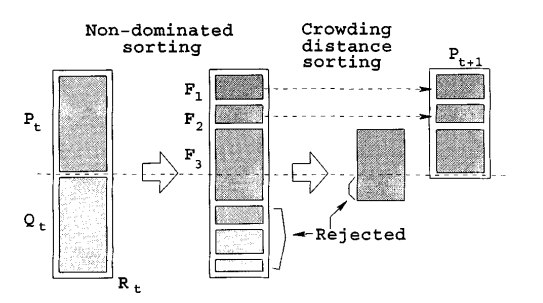
\includegraphics[width=\textwidth]{images/NSGA-2.PNG}
\caption{Thuật toán NSGA-II \cite{deb2002fast}}
\end{figure}
    \item Tiến hóa vi phân (\gls{DEs}): Tại bước khởi tạo, ngoài vecto khởi tạo ngẫu nhiên (gọi là genome hoặc chromosome), DEs có thêm vecto đột biến thu được bằng quá trình đột biến vi phân. Sau đó là qua trình lai ghép để tăng tính đa dạng cho quần thể. Các bước sau đó được  tiến hành như GAs
\end{itemize}
\emph{Giải thuật tối ưu dựa trên trí thông minh bầy đàn SIOAs}: Giải  thuật tối ưu dựa trên hành vi của các cá thể trong nhưng đơn vị xã hội nhỏ như bầy kiến, đàn chim,... Nhóm giải thuật này là một nhánh của trí tuệ nhân tạo (AI). 
\newline \emph{Mạng nơ ron nhân tạo (ANNs)}: Lấy cảm hứng từ mạng nơ-ron sinh học, mạng NN được hình thành từ các tầng nơ-ron nhân tạo. Mạng NN gồm ba kiểu tầng chính là tầng vào (input layer) biểu diễn cho đầu vào, tầng ra (output layer) biểu diễn cho kết quả đầu ra và tầng ẩn (hidden layer) thể hiện cho các bước suy luận trung gian. Mỗi nơ-ron sẽ nhận tất cả đầu vào từ các nơ-ron ở tầng trước đó và sử dụng một hàm kích hoạt (activation function) phi tuyến như sigmoid, ReLU,... để tính toán đầu ra. Trong mạng cảm biến không dây, mỗi nút cảm biến có thể được xem như một nơ-ron và cả mạng là một mạng nơ-ron nhân tạo. Tại mỗi nút cảm biến, ta có thể sử dụng ANNs để đưa ra hành động phù hợp cho nút cảm biến đó.
\newline \emph{Học tăng cường (RL)}: RL là một framework rất mạnh mẽ cho phép tác nhân (ở đây là các nút cảm biến) học thông qua tương tác với môi trường và cho phép mô hình hóa bài toán thành mô hình gọi là quá trình quyết định Markov, bao gồm:
\begin{itemize}
    \item Tác nhân
    \item Trạng thái
    \item Phần thưởng
    \item Hành động
\end{itemize}
Tại một thời điểm, tác nhân thực hiện một hành động và nhận được phần thưởng ứng với hành đông đó. Khi tác nhân đạt được mục tiêu, nó nhận được phần thưởng lớn nhất. 


\section{Bài toán}
Như đã trình bày tại mục 1.4 về các vấn đề trong \gls{WSNs}, vấn đề quan trọng và cơ bản nhất của mạng là tối ưu hóa bao phủ trong khi vẫn đảm bảo kết nối và tối ưu được thời gian sống của mạng. Ở đây, em muốn đề xuất một mô hình nhằm tối ưu cả ba mục tiêu trên.  Hơn nữa, để tăng tính chịu lỗi và khả năng giám sát của mạng, tối ưu bao phủ và kết nối ở đây là $k$-coverage và $c$-connectivity với $k$ và $c$ cho trước. Các mục tiêu này có sự  mâu thuẫn với nhau. Ví dụ, để đạt được mức độ bao phủ rộng hơn, các nút cảm biến phải được dàn rộng ra hơn trên khu vực mục tiêu. Điều này khiến năng lượng truyền thông tăng lên, các nút nhanh chóng cạn kiệt năng lượng hơn, tuổi thọ của mạng bị rút ngắn. Ngược lại, nếu muốn tăng tuổi thọ của mạng, các nút cần được đặt gần nhau hơn, gây ảnh hưởng đến phạm vi phủ sóng của mạng. Do vậy, trong bài toán này, em sẽ giải quyêt theo hai pha. Pha đầu tiên, tối ưu bao phủ và kết nối, pha sau thực hiện tối ưu thời gian sống. Kết quả của hai pha là một biên Pareto gồm các lời giải không thống trị lẫn nhau. 
\subsection{Mô hình hóa bài toán}
Bài toán có các đầu vào như sau:
\begin{itemize}
    \item $A$: Khu vưc mục tiêu được chia thành các ô lưới,  kích thước $mxn$
    \item $S$ = \{$s_1, s_2,..., s_n $\}: Tập các cảm biến
    \item $R_s$: Bán kính cảm biến 
    \item $R_c$: Bán kính truyền thông. Một nút cảm biến có thể truyền và nhận dữ liệu với các nút cảm biến nằm trong bán kính truyền thông của nó.
    \item $E$ = \{$e_1, e_2,..., e_m$\}: Tập các điểm mục tiêu (các điểm cần bao phủ). Trong bài toán, tập $E$ được chọn là giao điểm của các đường lưới. Điểm $e_i$ gọi là được bao phủ nếu $\exists s_j \in S, d(e_i, s_j) \leq R_s$
    \item Tập vị trí có thể rải cảm biến $P = \{p_1, p_2,..., p_3\}$. Vị trí rải cảm biến nằm trong khu vực mục tiêu A
    \item $ cov(e_i) = \{s_j | d(e_i, s_j) \leq R_s\}$ là tập các cảm biến bao phủ được điểm mục tiêu $e_i$
    \item $ tCov(s_j) = \{e_i | d(e_i, s_j) \leq R_s\}$ là tập các điểm mục tiêu nằm trong phạm vi cảm biến của nút cảm biến $s_j$
    \item $ con(s_i) = \{s_j | d(s_j, s_i) \leq R_c\}$ là tập các cảm biến có thể trao đổi thông tin với nút cảm biến $s_i$
    \item $E_{init}$ là năng lượng ban đầu các nút cảm biến được cung cấp.
\end{itemize}
Bài toán bao gồm ba mục tiêu như sau:
\begin{itemize}
    \item Mục tiêu thứ nhất: đảm bảo $k$-coverage
    \newline Xác suất một điểm mục tiêu $e_i$ được bao phủ bởi $k$ cảm biến được định nghĩa như sau:
    \begin{equation}
        covPro(e_i) = 
        \begin{cases}
            1 & \text{Nếu } |cov(e_i)| \geq k \\
            \frac{|cov(e_i)|}{k} & \text{Ngược lại}\\
        \end{cases}
    \end{equation}
    Do đó, mục tiêu đầu tiên có thể được biểu diễn toán học như sau:
    $$ Maximize f_1 = \frac{\sum_{i=1}^{m}covPro(e_i)}{m} $$
    
    \item Mục tiêu thứ hai: tối ưu xác suất $c$-connectivity
    \newline Xác suất một nút cảm biến $s_i$ kết nối được với $c$  nút cảm biến khác:
    \begin{equation}
        comPro(s_i) = 
        \begin{cases}
            1 & \text{Nếu } |com(s_i)| \geq c \\
            \frac{|com(s_i)|}{k} & \text{Ngược lại}\\
        \end{cases}
    \end{equation}
    Mục tiêu thứ hai được biểu diễn như sau:
    $$ Maximize f_2 = \frac{\sum_{i=1}^{n}comPro(s_i)}{n}$$
    
    \item Mục tiêu thứ 3 là đảm bảo hiệu quả năng lượng, kéo dài thời gian sống của mạng.
    \newline Năng lượng tiêu thụ để truyền l bit dữ liệu trên khoảng cách $d$ được tính bởi công thức:
    \begin{equation}
        E_t(l, d) = 
        \begin{cases}
            l * E_{elec} + l * \epsilon_{fs} * d^2 & d \geq d_0\\
            l * E_{elec} + l * \epsilon_{mp} * d^4 & d < d_0 \\
        \end{cases}
    \end{equation}
    Năng lượng để nhận được gói tin:
    $$ E_r = l * E_{elec}$$
    Do đó, năng lượng để một nút cảm biến $s_i$ nhận dữ liệu từ $num_i$ nút con và truyền dữ liệu đó tới nút cha $s_j$ được tính như sau:
    $$ E_{Ci} = E_t(l, d) + (E_{DA} + E_r(l))*num_i$$
    với:
    \begin{itemize}
        \item $d$ là khoảng cách từ nút $s_i$ đến nút cha $s_j$
        \item $E_{elec}$ là năng lượng tiêu tán để chạy thiết bị phát và thu trên nút cảm biến
        \item $\epsilon_{fs}$ là hệ số truyền năng lượng ở khoảng cách gần
        \item $\epsilon_{mp}$ là hệ số truyền năng lượng ở khoảng cách xa để đảm bảo một tỷ lệ lỗi bit có thể chấp nhận được
        \item $E_{DA}$ làn năng lượng tiêu tốn để tổng hợp dữ liệu.
    \end{itemize}
    Tuối thọ của một nút được tính bằng công thức:
    $$ L_i = \frac{E_{init}}{E_{Ci}}$$
    Vậy mục tiêu thứ ba là tối ưu hóa tuổi thọ của mạng:
    $$ Maximize f_3 = \frac{\sum_{i=1}^n L_i}{n} $$
    Một số hằng số tham khảo được cho ở bảng dưới:
    \begin{center}
    \begin{tabular}{ |c|c| } 
     \hline
     Tham số & giá trị  \\ 
     $E_{elec}$ & $50nJ/bit$  \\ 
     $\epsilon_{fs}$ & $10pJ/bit/m^2$  \\
     $\epsilon_{mp}$ & $0.0013pJ/bit/m^2$  \\
     $E_{DA}$ & $5pJ/bit$   \\
     \hline
    \end{tabular}
    \end{center}
\end{itemize}
Đầu ra của bài toán: Các vị trí được chọn để đặt các nút cảm biến $p_i \in P$
\subsection{Một số nghiên cứu liên quan}
Vấn đề tối ưu hóa đa mục tiêu trong mạng cảm biến không dây được nghiên cứu rộng rãi trong nhiều năm qua. Dưới đây em xin trình bày tóm tắt một số nghiên cứu liên quan đến tối ưu bao phủ, kết nối và thời gian sống của mạng:
\newline Nghiên cứu của Konstantinidis và các cộng sự \cite{konstantinidis2011multi} về triển khai mạng cảm biến  và vấn đề cấp phát năng lượng cho các nút cảm biến. Bài nghiên cứu sử dụng thuật toán \gls{MOEA/D} kết hợp với sáu phương pháp heuristic để cải thiện giá trị thích nghi của các cá thể qua các thế hệ. Đầu ra của bài toán là vị trí của các nút cảm biến $(x_j, y_j)$ và mức năng lượng $P_j$ gán cho nút. Hai mục tiêu cần tối ưu là  thời gian sống và độ bao phủ, với ràng buộc tất cả các nút đều được kết nối. Trong một nghiên cứu khác \cite{konstantinidis2011multi2}, các tác giả giải quyết bài toán với hai mục tiêu tương tự với ràng buộc chặt chẽ hơn là $k$-connectivity. Để đảm bảo ràng buộc này, bài báo đề xuất phương pháp sửa chữa cá thể bằng heuristic. Đóng góp của Konstantinidis là đã sử dụng được cả hai biến vị trí $(x_j, y_j)$ và mức năng lượng $P_j$ để tối ưu đồng thời cả thời gian sống và tuổi thọ của mạng. Các tác giả trước đó hầu như chỉ sử dụng một trong hai biến số để tối ưu hoặc là thời gian sống, hoặc là bao phủ.
\newline Nghiên cứu của Gupta và các cộng sự \cite{gupta2016genetic}: Sử dụng giải thuật di truyền (\gls{GAs}) để mạng đạt được k-coverage và m-connectivity sao cho  số lượng nút cảm biến cần sử dụng phải là nhỏ nhất. Nghiên cứu này có các  ưu điểm là chỉ sử dụng \gls{GAs} nên dễ thực thi, quá trình đột biến và lai ghép luôn sinh ra các cá thể con hợp lệ nên không cần các phương pháp sửa chữa lại cá thể con. Hàm mục tiêu của bài toán là tổng có trọng số của ba mục tiêu: $Fitness = W1*F1 + W2*F2 + W3*F3$ với $W1 + W2 + W3 = 1$.
\newline Nghiên cứu của Sengupta và các cộng sự \cite{sengupta2013multi}: Các tác giả nghiên cứu cách triển khai các nút cảm biến sao cho đảm bảo một loạt các yêu cầu của \gls{WSNs} như sau: 
\begin{itemize}
    \item Tối thiểu hóa số nút cảm biển cần thiết.
    \item Tối thiểu hóa tổng năng lượng tiêu thụ bởi các nút được triển khai.
    \item Tối đa vùng phủ sóng của mạng để tất cả các sự kiện xảy ra trong khu vực mục tiêu đều được phát hiện.
    \item Tối đa thời gian sống của mạng. 
\end{itemize}
Các tác giả mô hình hóa bài toán thành hai hàm mục tiêu cần tối thiểu hóa là: Hàm $f_1 = \sum_{i \in S}e_i$ là tổng năng lượng tiêu thụ của các nút, hàm $f_2 = \sum_{j \in D}NC_j * h_j$ với $NC_j$ là điểm phạt nếu điểm mục tiêu không được bao phủ (khi $h_j = 1$). Cùng với hai hàm mục tiêu này, các tác giả cũng đưa ra hai hàm buộc khác để đảm bảo kết nối trong mạng. Các tác giả thực hiện tối ưu hóa hai hàm mục tiêu với các trường hợp số lượng nút khác nhau để xem xét sự thay đổi của thời gian sống và năng lượng. Từ biên Pareto thu được, sử dụng một số kỹ thuật ra quyết định nhất định để chọn cách triển khai mạng thích hợp nhất. Bài toán được giải quyết theo cả hướng đơn mục tiêu (hàm $f2$ được sử dụng là hàm ràng buộc) và hướng đa mục tiêu, sử dụng thuật toán MOEA/DFD (là sự kết hợp của \gls{MOEA/D} với fuzzy dominance). Thông qua nghiên cứu này, ta có thể thấy hướng tiếp cận đa mục tiêu tốt hơn rất nhiều so với hướng giải bằng đơn mục tiêu trong việc tối thiểu hóa năng lượng, tăng tuổi thọ của mạng. Đồng thời, MOEA/DFD cũng cho kết quả tốt hơn \gls{MOEA/D} và \gls{NSGA-II} trong hầu hết các trường hợp khi so sánh về mức độ bao phủ.
\newline Trong các mô hình kể trên, các tác giả đều sử dụng các giải thuật tối ưu đa mục tiêu để tối ưu đồng thời các hàm mục tiêu. Để tránh phải tối ưu quá nhiều hàm mục tiêu cùng lúc, hàm kết nối thường được chọn là hàm ràng buộc. Trong đồ án này, em giải bài toán theo hướng chia thành hai pha riêng biệt. Pha đầu tiên có mục tiêu tối ưu $k$-coverage và $c$-connectivity. Pha thứ hai tối ưu thời gian sống bằng cách chọn đường đi thích hợp để truyền về trạm cơ sở cho các nút. Nhờ vậy, có thể tránh được việc tối ưu hai mục tiêu rất mâu thuẫn với nhau là thời gian sống và bao phủ và sử dụng được những giải thuật khác nhau phù hợp cho từng pha. Trong cả hai pha, các cá thể con sinh ra đều hợp lệ nên không cần bước sửa chữa. Cách làm chi tiết sẽ được trình bày ở mục 3.2.

\section{Sử dụng \gls{MOEA/D} cho mô hình bài toán đề xuất}
\subsection{Framework của MOEA/D}
\gls{MOEA/D} \cite{zhang2007moea} chia một bài toán đa mục tiêu thành $m$ bài toán con đơn mục tiêu bằng một số phương pháp tiếp cận như sử dụng tổng trọng số, Tchebycheff,... Cách chia theo tổng trọng số, một bài toán con đơn mục tiêu được định nghĩa như sau:
\begin{equation}
    max \quad g_i(x, \lambda) =  \sum_{i=1}^m \lambda_i f_i(x)
\end{equation}
với $\lambda = (\lambda_i,..., \lambda_m)$ là vecto trọng số, $\sum_{i=1}^m\lambda_i = 1$. Vecto này cho biết mức độ quan trọng của mỗi hàm mục tiêu trong một bài toán con. 
Thông thường, \gls{MOEA/D} bao gồm các bước sau:
Đầu vào:
\begin{itemize}
    \item $N$: số lượng bài toán con, đồng thời là số lượng cá thể trong quần thể.
    \item $N$ vecto trọng số $\lambda^1,..., \lambda^N$ được sinh theo phân phối đều.
    \item $T$ là số lượng bài toán con được coi là hàng xóm của bài toán con thứ $i$. Cần lựa chọn $T$ thật cẩn thận, nếu $T$ quá nhỏ, tại bước 2, cá thể con sinh ra quá giống cá thể cha mẹ, làm cho không gian tìm kiếm không được mở rộng. Tuy nhiên nếu $T$ quá lớn, các bài toán con không thực sự gần nhau sẽ làm cá thể con kém hiệu quả với bài toán con đang xét.
\end{itemize}
Các bước thực hiện
\begin{itemize}
    \item Bước 1: Khởi tạo
    \begin{itemize}
        \item Khởi tạo $EP = \emptyset$
        \item Tính toán khoảng cách Euclidean giữa các thành phần của vecto $\lambda$. Với mỗi $\lambda_i$, tìm tập $B(i) = \{i_1,..., i_\tau\} $ sao cho $\lambda_i,..., \lambda_\tau$ là $T$ vecto $\lambda$ gần $\lambda_i$ nhất. Tập $B(i)$ là tập gồm các bài toán con gần với bài toán con thứ $i$ nhất. Tất nhiên, vecto trọng số gần với $\lambda^i$ nhất là chính nó (khoảng cách bằng $0$), do đó, $i \in B(i)$. 
        \item Khởi tạo quần thể $x_1,.., x_N$, tính toán $F(x_i)$
    \end{itemize}
    \item Bước 2: Cập nhật
    Với mỗi cá thể thứ i trong quần thể:
    \begin{itemize}
        \item Chọn ngẫu nhiên $k, l \in B(i)$, sử dụng các phương pháp lai ghép, đột biến trên $x^k$ và $x^l$ để tạo ra cá thể con $y$. Do $x^k$ và $x^l$ đang là lời giải tốt nhất cho các bài toán con gần với bài toán con thứ $i$ nhất, nên ta có thể kỳ vọng $y$ sẽ là lời giải tốt cho bài toán con thứ $i$.
        \item Sau khi lai ghép, đột biến,... cá thể $y$ có thể trở nên bất hợp lệ (cấu trúc cá thể không hợp lệ) hoặc cần cải tiến, tối ưu. Do đó, ta cần sử dụng một số phương pháp heuristic nhất định để sửa chữa hoặc cải tiến $y$ thành  $y^{'}$
        \item Cập nhật các cá thể hàng xóm: $\forall j \in B(i) \text{ nếu } g(x_j, \lambda_j) < g(y^{'}, \lambda_i)$ thì $x_j = y^{'}, FV_j = F(y^{'})$. Do tập $B(i)$ gồm các bài toán con gần với bài toán con thứ $i$ nhất nên lời giải $y{'}$ có thể cũng sẽ tốt cho các bài toán này.
        \item Cập nhật EP: 
        \newline Loại bỏ khỏi EP những cá thể bị thống trị bởi $y{'}$
        \newline Thêm $y{'}$ vào EP nếu $y{'}$ không bị thống trị bởi bất cứ cá thể nào trong EP
    \end{itemize}
    \item Bước 3: Nếu đã đạt điều kiện dừng thì dừng lại, trả về EP. Nếu không, quay lại bước 2.
\end{itemize}
\subsection{Cách tiếp cận và lời giải cho mô hình bài toán đề xuất}
Phần này em xin trình bày cách giải cho mô hình bài toán đã đề cập tại chương 2 sử dụng \gls{MOEA/D}. Bài toán cần tối ưu ba yếu tố của mạng cảm biến không dây là: k-coverage, c-connectivity và tuổi thọ của mạng. Để đơn giản hóa, ta chia bài toán thành hai pha, tương ứng với 2 bài toán để giải. 
\begin{itemize}
    \item Pha 1: dùng MOEA/D để tối ưu đồng thời hai mục tiêu là bao phủ và kết nối. Kết thúc pha này ta nhận được đồ thị với các đỉnh là các nút cảm biến, các cạnh có đầu mút là hai nút cảm biến có thể gửi nhận dữ liệu với nhau.
    \item Pha 2: dùng \gls{GAs} để tìm đường đi tối ưu cho các nút cảm biển truyền về trạm cơ sở sao cho thời gian sống của mạng là lớn nhất.
\end{itemize}
Cụ thể cách làm như sau:
\subsubsection{Pha 1}
Thực hiện theo framework \gls{MOEA/D} đã trình bày ở trên, em xin chỉ trình bày lại một số bước cần mô tả chi tiết hơn.
\newline \emph{Biểu diễn cá thể}
Mỗi cá thể được biểu diễn bởi một mảng $n$ phần tử ($n$ là số lượng cảm biến). Giá trị mỗi phần tử là vị trí mà nút cảm biến đó được đặt vào. Ví dụ với $A[i] = j$, có thể hiểu là nút cảm biến $s_i$ được đặt ở vị trí $p_j$. Do không đặt các nút cảm biến cùng một vị trí nên $A[i] \neq A[j], \text{ } \forall i \neq j$, tức là các gen của cùng một cá thể phải khác nhau.
\newline \emph{Lai ghép và đột biến}
Phương pháp lai ghép được sử dụng là lai ghép một điểm cắt (one point crossover). Điểm lai ghép được lựa chọn ngẫu nhiên, cá thể con có đoạn đầu (tính từ đầu đến điểm lai ghép) của cá thể bố và phần sau của cá thể mẹ. Đối với đoạn sau,  ta cần duyệt lần lượt các gen của cá thể mẹ, và chỉ thêm vào cá thể con các gen mà cá thể con chưa có.
\begin{lstlisting}
    def crossover(indi1, indi2):
      crossoverPoint = random.randint(0, NUMBER_OF_SENSORS - 1)
      child = list(indi1[:crossoverPoint])
      index = [j for j in indi2 if j not in child]
      for i in range(NUMBER_OF_SENSORS - crossoverPoint):
        child.append(index[i])
    return np.array((child))
\end{lstlisting}
Để đột biến cá thể con, ta chọn ngẫu nhiên một số vị trí trong gen rồi thay đổi giá trị của vị trí đó.
\newline \emph{Hàm tính toán giá trị thích nghi}
Đầu tiên, tính toán giá trị bao phủ $f_1$ và giá trị kết nối $f_2$ của cá thể theo công thức đã đề cập trong mục 2.1. Mức độ thích nghi của cá thể $x_i$ được đánh giá bởi:
\begin{equation}
    F = \lambda_i*f_1(x_i) + (1-\lambda_i)*f_2(x_i)
\end{equation}

\subsubsection{Pha 2}
Pha này liên quan đến nhiều thao tác, thuật toán trên đồ thị nên em sử dụng thư viện NetworkX \cite{hagberg2008exploring} để thực hiện. NetworkX là một thư viện Python rất hữu ích khi làm việc với đồ thị, xử lý được  nhiều dạng cấu trúc  (vô hướng, có hướng, đa đồ thị), cung cấp sẵn các thuật toán đồ thị thông dụng như Kruskal, Prim...
Pha 2 có đầu vào là đồ thị G có tập đỉnh $V = S$ và tập cạnh $E = {(s_i, s_j) | d(s_i, s_j) <= r_c}$, trọng số các cạnh là $d(s_i, s_j)$. Đâu ra là một biên Pareto gồm các cây khung cho thời gian sống $f_3$ tối ưu nhất.
Để biểu diễn các cá thể con có dạng cây, em sử dụng cách mã hóa Link and node biased encoding được đề xuất trong \cite{palmer1994representing}.
\newline \emph{Mã hóa}: Trong cách biểu diễn này, mỗi cá thể là một chuỗi gồm $|V|$ giá trị bias cho $|V|$ đỉnh và $|E|$ giá trị bias cho $|E|$ cạnh. Ví dụ, một đồ thị như hình vẽ dưới được biểu diễn là [b1, b2, b3, b4, b12, b13, b34]. 
\begin{figure}[ht]
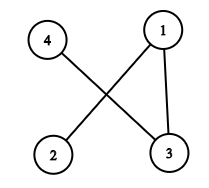
\includegraphics[width=0.5\textwidth]{images/graph.PNG}
\end{figure}
Các giá trị bias cho cạnh $b_{ij}$ giúp cho cách mã hóa này có thể biểu diễn được mọi cây T nếu có giá trị bias phù hợp.
Ta sẽ tính toán lại giá trị trọng số cho đồ thị theo công thức:
\begin{equation}
    C^{'}_{ij} = C_{ij} + P_1*C_{max}*b_{ij} + P_2*C_{max}*{b_i + b_j}
\end{equation}
với $C_max$ là trọng số lớn nhất của đồ thị.
\newline \emph{Giải mã}:  Cây khung mà cá thể biểu diễn thu được bằng cách áp dụng thuật toán tìm cây khung nhỏ nhất (ví dụ như Prim). Sau đó MST này được đánh giá giá trị thích nghi thông qua các giá trị trọng số ban đầu.
\newline Đối với bài toán cần giải, chọn $P_1 = P_2 = 1$ và $b \in [0; 255]$
\newline Chọn lọc: Sử dụng thuật toán Bánh xe Roulette (Roulette Wheel Selection) như sau:
\begin{itemize}
    \item Sắp xếp quần thể theo thứ tự giảm dần giá trị thích nghi
    \item Tính tổng giá trị thích nghi của cả quần thể
    \item Tính tổng tích lũy của mỗi cá thể: $cumsum(x_i) = f_3(x_i) + f_3(x_{i-1}) $
    \item Sinh giá trị ngẫu nhiên $r$ trong đoạn [0, 1)
    \item Nếu cá thể $x_i$ có $cumsum(x_i) \geq r$ thì cá thể $x_i$ được chọn 
\end{itemize}
Các cá thể được chọn lọc ra tạo thành một tập gọi là $ mating pool$. Thực hiện lai ghép một điểm cắt trên tập này ta thu được quần thể con $breedPopulation$. Sau đó, thực hiện đột biến trên các gen bất kỳ để thu được quần thể con đột biến $mutatedPopulation$. Tiếp theo kết hợp 2 quần thể này với quần thể ban đầu, ta thu được quần thể $Q$.
\newline Sắp xếp quần thể Q theo thứ tự giảm dần của giá trị thích nghi và thực hiện chọn lọc theo thuật toán Roulette Wheel để chọn các cá thể cho thế hệ sau. Tại đây, để đảm bảo các cá thể tốt nhất (có giá trị thích nghi cao) chắc chắn được chọn lọc vào thế hệ sau, đồng thời đảm bảo sự đa dạng của quần thể, 90\% của quần thể được chọn lọc nhờ thuật toán Roulette Wheel và 10\% còn lại là các cá thể có giá trị thích nghi lớn nhất của quần thể trước.

\section{Kết quả thực nghiệm}

\newpage
\bibliographystyle{unsrt} % We choose the "plain" reference style
\bibliography{refs} % Entries are in the "refs.bib" file

\end{document}
